\documentclass[onlymath,xcolor=pdftex,dvipsnames,table]{beamer}
\usefonttheme{serif}

\usepackage{array}
\usepackage{color}
\usepackage{xspace}
\usepackage{graphicx}
\usepackage{subfigure}
\usepackage{pstricks}
\usepackage{booktabs}
\usepackage{listings}
\usepackage{multimedia}
%\usepackage{beamerthemeshadow}
\usepackage{amsmath,amsfonts,amsthm,amssymb}
\usepackage[noend]{algpseudocode}
\usepackage{algorithm}
\usepackage{algorithmicx}
\usepackage{transparent} % transparent background
\usepackage{etoolbox}

\usetheme{Singapore}
%\usefonttheme{serif}
%\useoutertheme{infolines}
%\setbeamertemplate{background canvas}[vertical shading]
%				     [bottom=red!10,top=blue!10]

%---------- header setting ------------------------------------------------%
% a flag that tells us how the circles should be drawn
\newif\ifnavbeforecurrent
% reset the flag before every navigation bar
\pretocmd\insertnavigation{\navbeforecurrenttrue}{}{}

% change the circle drawing code so that it changes based on the flag
\defbeamertemplate*{mini frame in current subsection}{changing}[1][50]
{%
  \begin{pgfpicture}{0pt}{0pt}{0.1cm}{0.1cm}
    \pgfpathcircle{\pgfpoint{0.05cm}{0.05cm}}{0.05cm}
    \ifnavbeforecurrent
        \pgfusepath{fill,stroke}
    \else
        \pgfusepath{stroke}
    \fi
  \end{pgfpicture}%
}
\setbeamertemplate{mini frame in current subsection}[changing]

% after the circle for the current frame is drawn, change the flag
\defbeamertemplate*{mini frame}{changing}
{%
  \begin{pgfpicture}{0pt}{0pt}{0.1cm}{0.1cm}
    \pgfpathcircle{\pgfpoint{0.05cm}{0.05cm}}{0.05cm}
    \pgfusepath{fill,stroke}
  \end{pgfpicture}%
  \global\navbeforecurrentfalse
}
\setbeamertemplate{mini frame}[changing]

%---------- footer setting ------------------------------------------------%
\makeatletter
\setbeamertemplate{footline}
{
  \leavevmode%
  \hbox{%
  %\begin{beamercolorbox}[wd=.333333\paperwidth,ht=2.25ex,dp=2ex,center]{author in head/foot}%
  %  \usebeamerfont{author in head/foot}%
  %\insertshortauthor\hspace{1em}\beamer@ifempty{\insertshortinstitute}{}{(\insertshortinstitute)}
  %\end{beamercolorbox}%
  \begin{beamercolorbox}[wd=.5\paperwidth,ht=2.25ex,dp=2ex,left]{title in head/foot}%
    \usebeamerfont{title in head/foot}\hspace{1em}\insertshorttitle
  \end{beamercolorbox}%
  \begin{beamercolorbox}[wd=.5\paperwidth,ht=2.25ex,dp=2ex,right]{date in head/foot}%
    \usebeamerfont{date in head/foot}\insertshortdate{}\hspace*{2ex}
    %\insertframenumber{}/\inserttotalframenumber\hspace*{2ex} 
  \end{beamercolorbox}}%
  \vskip0pt%
}
\makeatother
% no navigation bar
\beamertemplatenavigationsymbolsempty
% only page number version below
%\setbeamertemplate{footline}[page number]

%---------- footnote setting ------------------------------------------------
\addtobeamertemplate{footnote}{\vspace{-6pt}\advance\hsize-0.5cm}{\vspace{6pt}}
\makeatletter
% Alternative A: footnote rule
\renewcommand*{\footnoterule}{\kern -3pt \hrule \@width 2in \kern 8.6pt}
% Alternative B: no footnote rule
% \renewcommand*{\footnoterule}{\kern 6pt}
\makeatother

{\setbeamertemplate{background canvas}{%
  %\begin{picture}(0,0)
  %  \put(302,-240){
  %    \includegraphics[width=0.15\paperwidth]{owl.jpg}}
  %\end{picture}}
\frame{\titlepage}}}

%---------- User-defined commands -----------------------------------------%
\newcommand{\probkb}{\textsc{ProbKB}\xspace}
\newcommand{\sherlock}{\textsc{Sherlock}\xspace}
\newcommand{\holmes}{\textsc{Holmes}\xspace}
\newcommand{\reverb}{\textsc{ReVerb}\xspace}
\newcommand{\tuffy}{\textsc{Tuffy}\xspace}
\newcommand{\felix}{\textsc{Felix}\xspace}
\newcommand{\alchemy}{\textsc{Alchemy}\xspace}
\newcommand{\blog}{\textsc{Blog}\xspace}
\newcommand{\nell}{\textsc{Nell}\xspace}
\newcommand{\probase}{\textsc{ProBase}\xspace}
\newcommand{\textrunner}{\textsc{TextRunner}\xspace}
\newcommand{\madden}{\textsc{MADden}\xspace}
\newcommand{\gist}{\textsc{GIST}\xspace}

\definecolor{darkblue}{rgb}{0,0,0.6}
\definecolor{darkred}{rgb}{0.6,0,0}

\let\oldemph\emph
\renewcommand{\emph}[1]{{\color{Blue}\oldemph{#1}}}
\newcommand{\define}[1]{\textit{#1}\xspace}
\newcommand{\strong}[1]{\textbf{#1}\xspace}
\newcommand{\stt}[1]{\texttt{\small #1}\xspace}

\newcommand{\head}[1]{{\large\color{OliveGreen}#1\\[2pt]}}


% declaration of the new block
\algblock{ParFor}{EndParFor}
% customising the new block
\algnewcommand\algorithmicparfor{\textbf{for}}
\algnewcommand\algorithmicpardo{\textbf{do in parallel}}
\algnewcommand\algorithmicendparfor{\textbf{barrier end}}
\algrenewtext{ParFor}[1]{\algorithmicparfor\ #1\ \algorithmicpardo}
\algrenewtext{EndParFor}{\algorithmicendparfor}

\definecolor{lightgray}{rgb}{0.98,0.98,0.98}
\hypersetup{colorlinks,linkcolor=,urlcolor=Blue}

\renewcommand{\ttdefault}{pcr}
\lstset{
  language=SQL,
  basicstyle={\footnotesize\ttfamily},
  numbers=none,
  backgroundcolor=\color{lightgray},
  aboveskip=3mm,
  belowskip=3mm,
  showstringspaces=false,
  columns=flexible,
  keywordstyle={\bfseries\color{Blue}},
  commentstyle={\color{Red}\textit},
  stringstyle=\color{Magenta},
  frame=single,
  breaklines=true,
  breakatwhitespace=true,
  tabsize=4
}

\AtBeginSubsection[]
{
 \begin{frame}
   \frametitle{Outline}
   \tableofcontents[currentsection,currentsubsection]
 \end{frame}
}

%% \AtBeginSection[]
%% {
%%   \begin{frame}
%%     \frametitle{Outline}
%%     \tableofcontents[currentsection,currentsubsection]
%%   \end{frame}
%% }

%\newlength{\wideitemsep}
%\setlength{\wideitemsep}{\itemsep}
%\addtolength{\wideitemsep}{5pt}
%\let\olditem\item
%\renewcommand{\item}{\setlength{\itemsep}{\wideitemsep}\olditem}

\title[\probkb Web-Scale Probabilistic Knowledge Base]%(optional, only for long titles)
{\probkb Web-Scale\\Probabilistic Knowledge Base}
\author % (optional, for multiple authors)
{Yang~Chen, Xing~Liu\\{\footnotesize{\{yang,xinliu\}@cise.ufl.edu}}}
\institute[University of Florida] % (optional)
{
  Computer and Information Science and Engineering\\
  University of Florida\\
}
\date{Mar 12, 2013} % (optional)
\logo{
\includegraphics[width=3cm]{logo.pdf}}

\begin{document}

\maketitle

%---------- slide --------------------------------------------------%
\section{Introduction}
\subsection{Introduction}
\begin{frame}{Knowledge bases--Introduction}
\begin{itemize}
  \item A \emph{knowledge base} is a collection of entities, facts, and relationships that conforms with a certain data model.
  \item A knowledge base helps machines understand humans, languages, and the world.
\end{itemize}
\begin{figure}
  \centering
  \subfigure{
    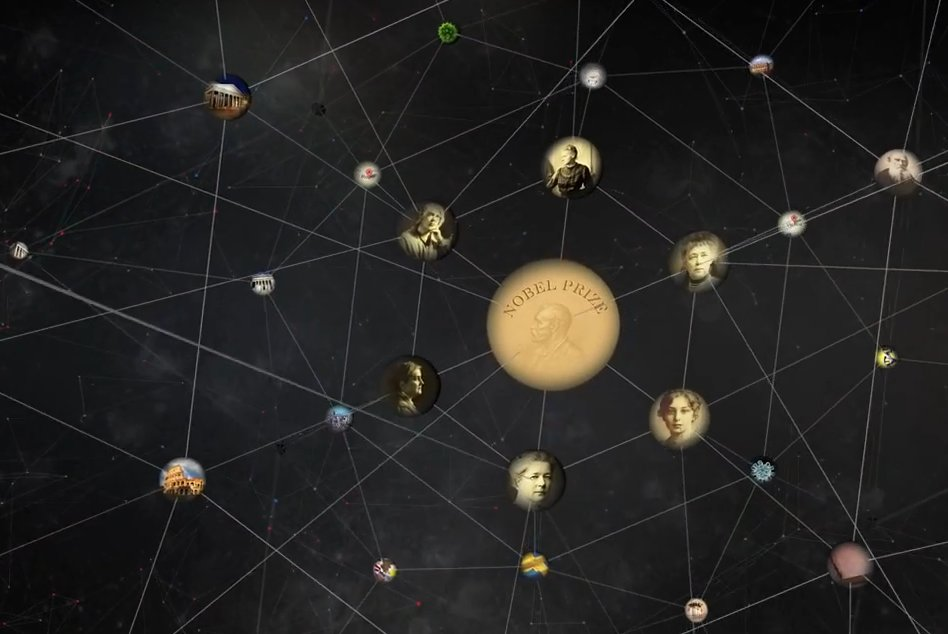
\includegraphics[width=.4\textwidth]{120701_google_knowledge_graph.jpg}   
    \label{fig:subfig1}
  }
  \subfigure{
    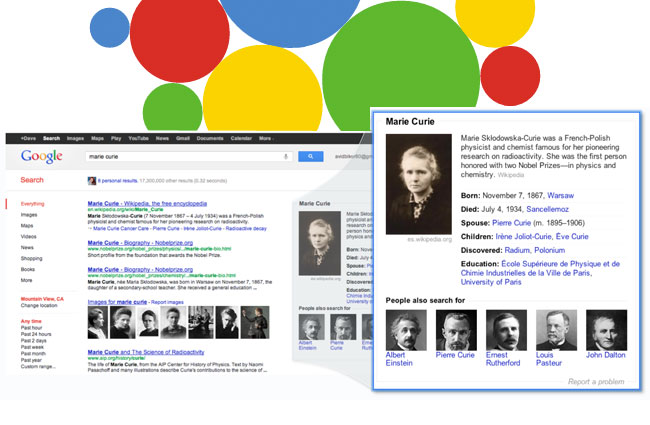
\includegraphics[width=.4\textwidth]{Google-Knowledge-Graph.jpg}   
    \label{fig:subfig1}
  }
  \caption{Google knowledge graph}
\end{figure}
\end{frame}


%---------- slide --------------------------------------------------%
{\usebackgroundtemplate{\put(210,-250){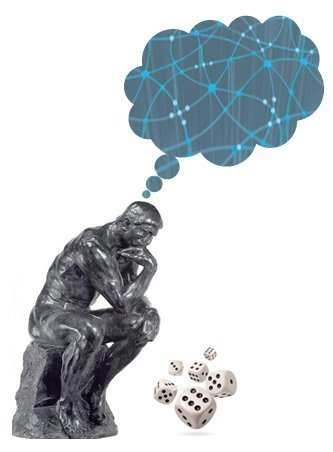
\includegraphics[width=.25\paperwidth]{pgm.jpg}}}
\begin{frame}{Challenges \& Motivation}
{\large Knowledge Acquisition}
\vspace{-30pt}
\begin{itemize}
  {\bfseries\color{red}
  \item Statistical Inference
    \begin{itemize}\color{red}
      \item Markov logic
    \end{itemize}}
  \item Information extraction
    \begin{itemize}
      \item NELL (CMU), OpenIE (UW)
      \item Entities, relations, rules
    \end{itemize}
  \item Human collaboration
    \begin{itemize}
      \item Wikipedia
      \item Freebase
    \end{itemize}
\end{itemize}
\end{frame}}


%---------- slide --------------------------------------------------%
{\usebackgroundtemplate{\put(210,-250){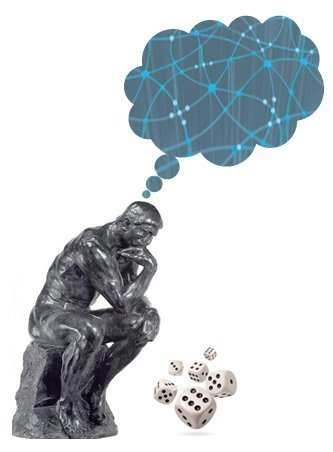
\includegraphics[width=.25\paperwidth]{pgm.jpg}}}
\begin{frame}{Challenges \& Motivation}
{\large Uncertainty Management}
\vspace{-30pt}
\begin{itemize}
  {\bfseries\color{red}
  \item Statistical Inference
    \begin{itemize}\color{red}
      \item Probabilistic graphical models
      \item Markov chain Monte Carlo
    \end{itemize}}
  \item Data integration
    \begin{itemize}
      \item Merging multiple data sources
      \item Crowdsourcing/user feedback
    \end{itemize}
  \item Data cleaning
    \begin{itemize}
      \item Conflict, incomplete, outdated data
    \end{itemize}
\end{itemize}
\end{frame}}


%---------- slide --------------------------------------------------%
{\usebackgroundtemplate{\put(210,-230){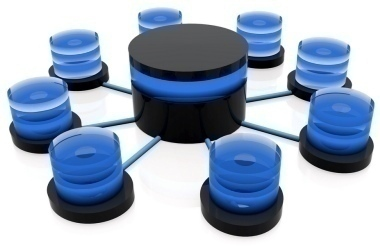
\includegraphics[width=.25\paperwidth]{db.jpg}}}
\begin{frame}{Challenges \& Motivation}
{\large Scalability}
\vspace{-30pt}
\begin{itemize}
  \item \textbf{\color{red}Scalable data management systems}
    \begin{itemize}
      \item \textbf{\color{red}Relational DBMS}
      \item Hadoop
      \item Spark, GraphLab, \textbf{\color{red}Datapath}, etc
    \end{itemize}
  \item Scalable algorithms
    \begin{itemize}
      \item Incremental inference
      \item Query-driven inference
    \end{itemize}
\end{itemize}
\end{frame}}


%---------- slide --------------------------------------------------%
\section{The \probkb System}
\subsection{\probkb Architecture}
\begin{frame}{Architecture}
\begin{figure}
  \centering
  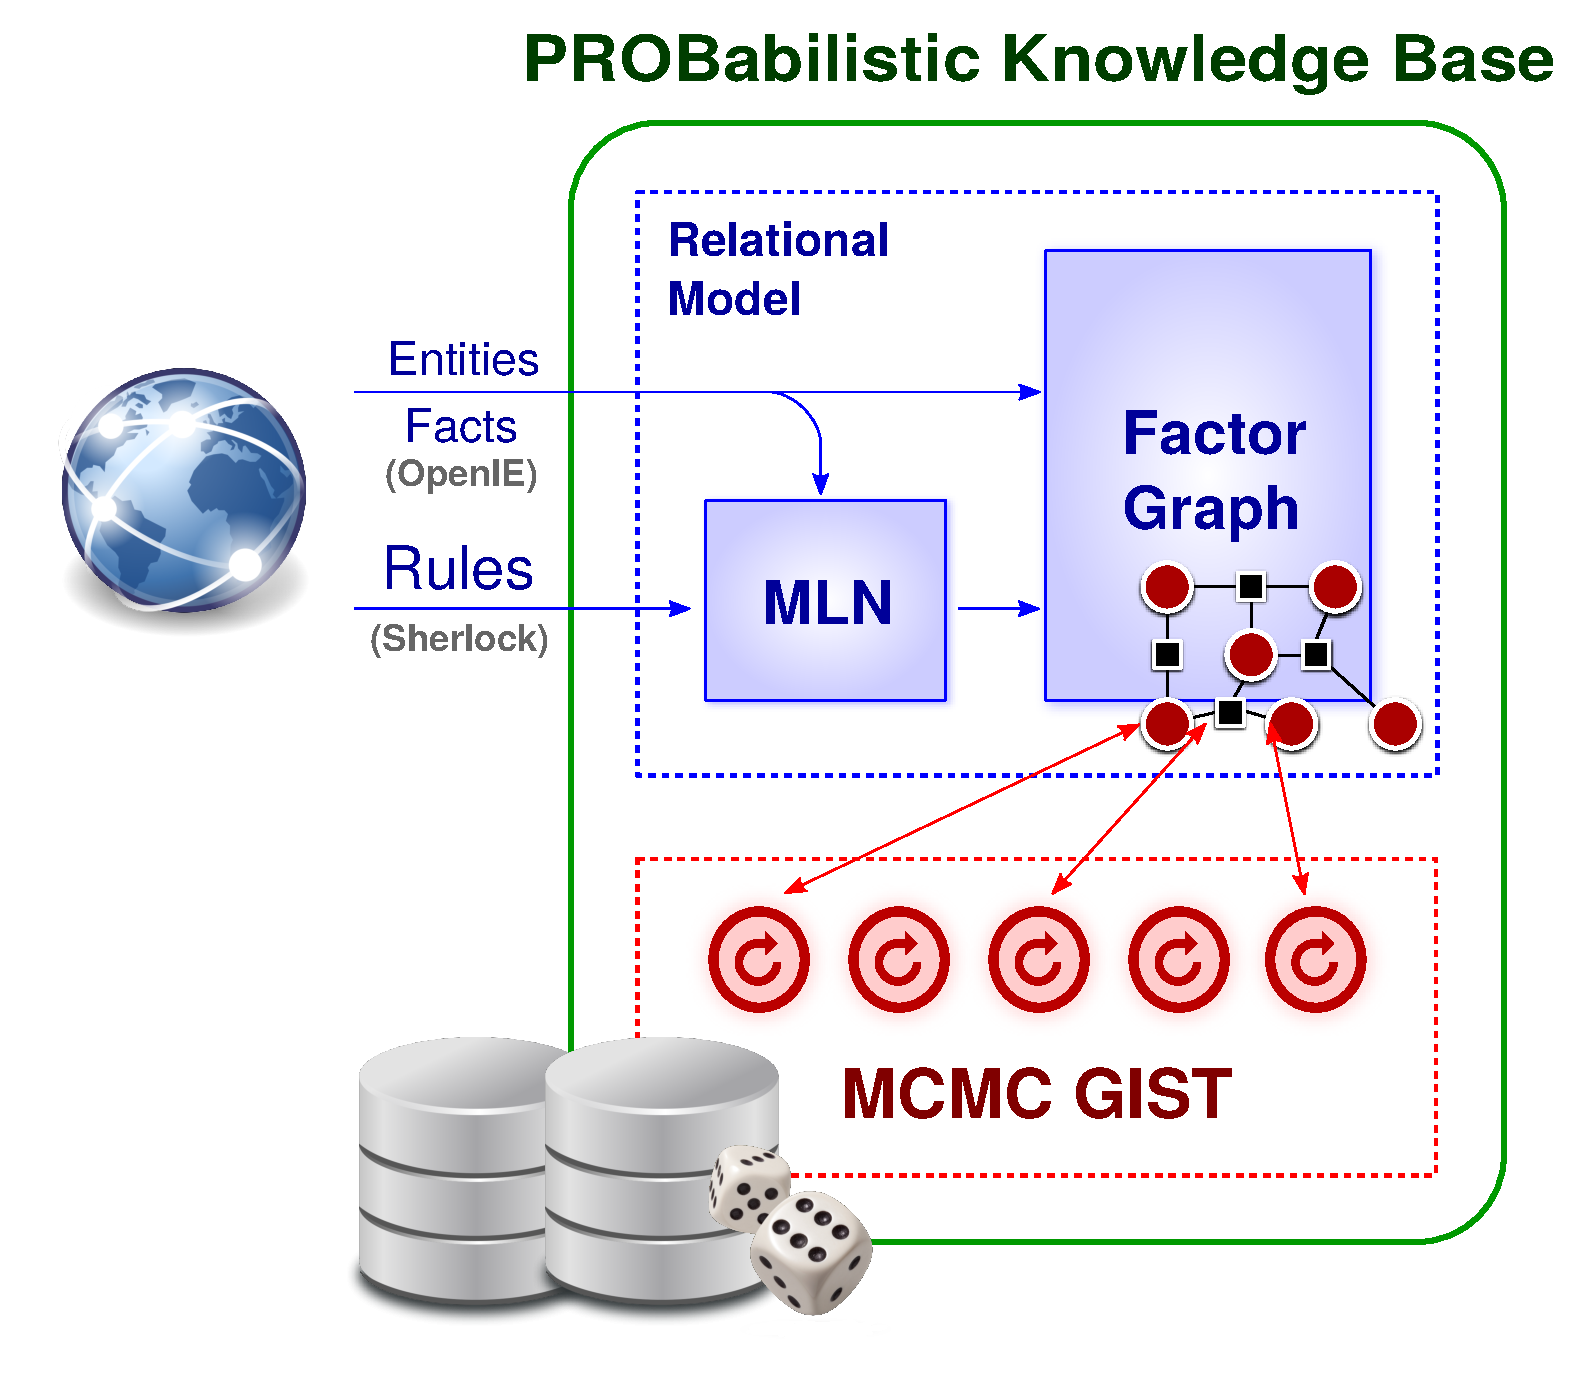
\includegraphics[clip,trim=30 0 15 0,width=.7\textwidth]{probkbarch.pdf}
\end{figure}
\end{frame}

%---------- slide --------------------------------------------------%
\begin{frame}{Markov Logic--Probabilistic Inference Framework}
A \emph{Markov logic network} (MLN) is a set of formulae with weights. Together with a finite set of constants $C=\{c_1,\ldots,c_{\left\vert C\right\vert}\}$, it defines a Markov network.

\begin{columns}[c]
  \column{0.48\textwidth}
  \begin{table}\tiny
    \centering
    \begin{tabular}{cc}\toprule
      \textbf{Weight} & \textbf{First-Order Logic}\\\midrule
      0.7 & Fr($x$,$y$)$\wedge$Fr($y$,$z$)$\rightarrow$Fr($x$,$z$)\\
      1.5 & Sm($x$)$\rightarrow$Ca($x$)\\
      1.1 & Fr($x$,$y$)$\wedge$Sm($x$)$\rightarrow$Sm($y$)\\
      \bottomrule
    \end{tabular}
    \caption{Example Markov logic network.}
    \label{tab:mln}
  \end{table}

  \column{0.48\textwidth}
  A set of constants (entities, or objects) $$C=\{A,B\}.$$
\end{columns}\vspace{-25pt}
\begin{figure}
  \centering
  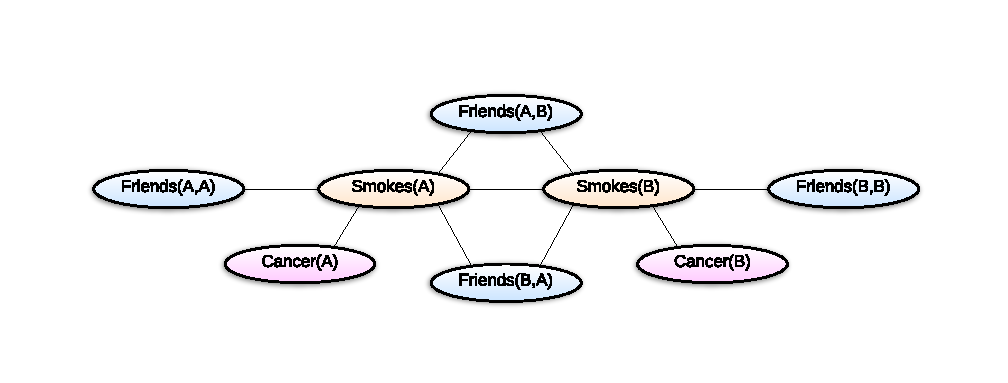
\includegraphics[clip,trim=40 35 40 40,width=0.75\textwidth]{mrf.pdf}
  \caption{Grounded Markov network.}
  \label{fig:ground}
\end{figure}
\end{frame}


%---------- slide --------------------------------------------------%
\subsection{Grounding}
\begin{frame}{Grounding}
\emph{Grounding} is the process of substituting constants into MLN clauses.\\[5pt]

The result of grounding is a \emph{factor graph} (or \emph{Markov network}) from which we can infer marginal probabilities for individual facts.\\[15pt]

\head{Key Challenges}
\begin{itemize}
  \item Time-consuming, especially if the numbers of rules and entites are large.
  \item Grounded network has an intractably large size, making inference tasks slow.
\end{itemize}
\end{frame}


%---------- slide --------------------------------------------------%
\begin{frame}{Markov Logic: A Relational Point of View}
\begin{itemize}
\item State-of-the-art (\tuffy, \nell): one table for each relation
\item By considering only Horn clauses, we store the rules and relationships in a few tables:
\end{itemize}
\vspace{-20pt}
\begin{columns}
  \column{.5\textwidth}
    \begin{table}[h]
      \centering
      \caption{\stt{MLN (M)}}
      \begin{tabular}{ccc}\toprule
        \stt{head} & \stt{body1} & \stt{body2}\\\midrule
        $p_1$ & $q_1$ & $r_1$\\
        $p_2$ & $q_2$ & $r_2$\\
        $p_3$ & $q_3$ & $r_3$\\
        $p_4$ & $q_4$ & $r_4$\\
        & $\cdots$ &\\
        \bottomrule
      \end{tabular}
    \end{table}

  \column{.5\textwidth}
    \begin{table}[h]
      \centering
      \caption{\stt{Relationships (R)}}
      \begin{tabular}{ccc}\toprule
        \stt{pred} & \stt{ent1} & \stt{ent2}\\\midrule
        $p_1$ & $x_1$ & $y_1$\\
        $p_1$ & $x_2$ & $y_2$\\
        $p_2$ & $x_1$ & $y_1$\\
        $p_2$ & $x_2$ & $y_2$\\
        & $\cdots$ &\\
        \bottomrule
      \end{tabular}
    \end{table}

\end{columns}
\end{frame}


%---------- slide --------------------------------------------------%
\begin{frame}{Markov Logic: A Relational Pointer of View}
The grounding of \emph{ALL} rules of form $$p(x,y)\leftarrow q(x,z), r(z,y)$$ is then expressed as a relational operation:
\begin{align}\small
R&\leftarrow\rho_{R(\stt{pred,ent1,ent2})}(\pi_{M.\stt{head}, R_2.\stt{ent1}, R_3.\stt{ent2}}\\\nonumber
&\phantom{\leftarrow}((M\bowtie_{M.\stt{body1}=R_2.\stt{pred}} R_2)\\\nonumber
&\phantom{\leftarrow}\bowtie_{M.\stt{body2}=R_3.\stt{pred} \stt{ AND } R_2.\stt{ent2}=R_3.\stt{ent1}} R_3))\nonumber\\
G&\leftarrow R_1\bowtie R\nonumber
\end{align}
\end{frame}


%---------- slide --------------------------------------------------%
\begin{frame}{Grounding Results}
The relational Markov logic model saves us from managing thousands of tables as in previous approaches. As a result, We grounded the whole \sherlock-\holmes dataset in about 1.5 hours using Greenplum, while the state-of-the-art implementation MLN crashes during its grouding phase.
\begin{table}
  \centering
  \rowcolors{1}{RoyalBlue!20}{RoyalBlue!5}
  \begin{tabular}{|c|c|}\hline
   \#relations & 10,672 \\
   \#rules     & 31,000 \\
   \#constants & 1.1M \\
   \#evidence  & 250,000 \\
   \#queries   & 10,672 \\
   \tuffy      & \textbf{\color{Red}Crash} \\
   \probkb     & 1.5 h\\
   \hline
  \end{tabular}
  \caption{Dataset statistics and performance.}
\end{table}
\end{frame}


%---------- slide --------------------------------------------------%
\subsection{Inference}
\begin{frame}{Inference: MCMC-MH}
\begin{figure}
  \centering
  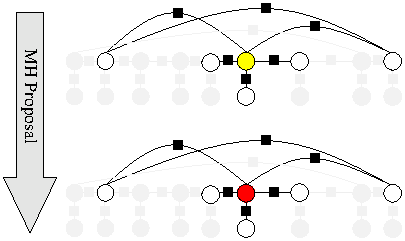
\includegraphics[width=.5\textwidth]{mcmc.pdf}
\end{figure}
Markov locality property allows for parallel computing.
\end{frame}


%---------- slide --------------------------------------------------%
\begin{frame}{Datapath \gist}
\head{Generalized Iterable State Transforms (GIST)}
\begin{itemize}
  \item GIST Performs \emph{transitions} upon a \emph{state} until that state has converged to the desired result.
  \begin{description}
    \item[Transition] MCMC Proposal function.
    \item[State] Factor graph with its samples.
  \end{description}
  \item A user-defined local scheduler allows general MCMC proposal implementation.
  \item The GIST state keeps track of the inference result.
\end{itemize}
\end{frame}


% New modification to parallel mcmc in datapath. %
%---------- slide --------------------------------------------------%
\begin{frame}{Datapath \gist}
\head{Parallel Mcmc implementation modification on datapath}
\begin{itemize}
  \item Previous approach: cut the graph to smaller graphs, run mcmc on each partition. 
    \begin{itemize}
      \item Lost information when a factor is accross multiple subgraphs.  Inaccurate, but the faster performance.
    \end{itemize}
  \item Modified approach: Do not cut the graph. Add write lock on each variables.
    \begin{itemize}
      \item More accurate, but lower performance. 
    \end{itemize}
\end{itemize}
\end{frame}


%---------- slide --------------------------------------------------%
\begin{frame}{Parallel mcmc with write lock in datapath}
\begin{figure}
  \centering
  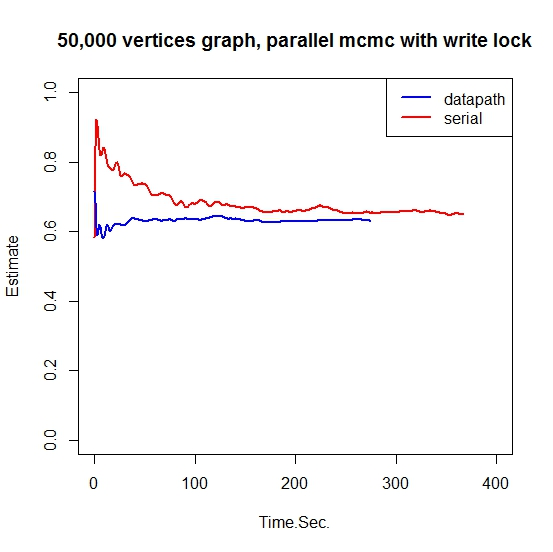
\includegraphics[width=.6\textwidth]{R1.jpeg}
\end{figure}
\end{frame}


%---------- slide --------------------------------------------------%
\begin{frame}{Parallel mcmc with write lock in datapath}
\begin{figure}
  \centering
  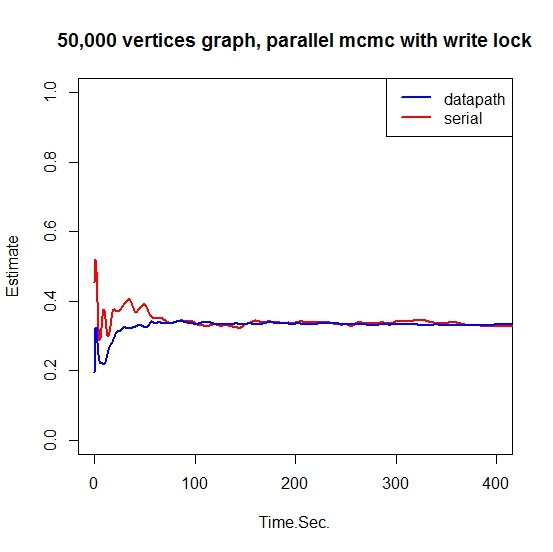
\includegraphics[width=.6\textwidth]{R3.jpeg}
\end{figure}
\end{frame}


%---------- slide --------------------------------------------------%
\begin{frame}{Preliminary Results}
\begin{table}[h]
  \centering
  \begin{tabular}{cccccc}\toprule
    \# Vertices & 5000	& 10,000 & 25,000 & 250,000 & 2,500,000\\\midrule
       Single Thread & 7 sec & 28 sec & 228 sec & Hours	& N/A\\
       Datapath & 7 sec & 13 sec & 30 sec & 2661 sec & N/A\\
     \bottomrule
  \end{tabular}
  \caption{Time to generate 5000 joint samples for different graphs.}
\end{table}
\end{frame}


%---------- slide --------------------------------------------------%
\section{Discussion}
\subsection{Discussion}
\begin{frame}{Next Steps}
\begin{itemize}
  \item Grounding/inference connection
    \begin{itemize}
      \item Construct graph structures from relational format.
      \item Partition and Merge: opportunity of GLA parallelism.
    \end{itemize}
  \item DB-memory synchronization
    \begin{itemize}
      \item Determine an update and write-back policy to synchronize DB and in-memory data.
      \item Buffer manager; IO efficiency
    \end{itemize}
  \item Incremental inference
    \begin{itemize}
      \item Schedule Datapath execution so that computation is focused on the least convergent portion of the factor graph.
    \end{itemize}
  \item Evaluation
    \begin{itemize}
      \item MCMC evaluation: multi-chain convergence test
      \item Result evaluation: Manual check (AMT)
    \end{itemize}
\end{itemize}
\end{frame}


%---------- slide --------------------------------------------------%
\begin{frame}{Responsibilities}
\begin{description}
  \item[Yang] Grounding
  \item[Xing] Inference
\end{description}
\end{frame}


%---------- slide --------------------------------------------------%
\begin{frame}{Questions?}
\begin{center}
  \LARGE Thank you!
\end{center}
\end{frame}


\end{document}
